\documentclass[11pt,letterpaper]{article}
\usepackage[margin=0.88in]{geometry}
\usepackage{booktabs,array,graphicx,xcolor,hyperref}
\definecolor{pine}{HTML}{194C40}
\hypersetup{colorlinks=true,urlcolor=pine,linkcolor=pine,pdftitle={DroidFork: Fresh Android Checkpoint Forks on Apple Silicon},pdfauthor={Nikit Phadke}}
\newcommand{\project}{\href{https://github.com/nikitph/droidfork}{DroidFork repository}}
\newcommand{\data}[2]{\href{https://github.com/nikitph/droidfork/blob/main/results/#1}{#2}}
\newcommand{\hd}[1]{\par\vspace{9pt}{\large\bfseries\color{pine} #1}\par\smallskip}
\setlength{\parindent}{0pt}\setlength{\parskip}{5pt}
\linespread{1.04}
\begin{document}
{\small\sffamily\color{pine} SYSTEMS RESEARCH NOTE \hfill 20 NOVEMBER 2026}\par
\vspace{12pt}{\Huge\bfseries DroidFork}\par
{\LARGE Fresh Android checkpoint forks on Apple Silicon}\par
\vspace{5pt}Nikit Phadke \quad $\cdot$ \quad \project\par
\hd{Abstract}
Branching an agent trajectory requires reproducing intermediate application state and accepting the next action. We measure that operation end to end on an Apple M1 Pro. A modified Android Emulator creates a fresh child from a saved Contacts draft, injects a touchscreen event, and returns a live accessibility hierarchy and a rendered image. The fastest verified request took 1.145\,s. Across six repeat native-touchscreen launches, every request passed and the median was 1.233\,s. The child had no process, private disk or reserved VM at request time. Read-only checkpoint preparation and ordinary filesystem caching were allowed. The measurements cover one offline task and one host.
\hd{1\quad The timing contract}
A trainer has reached an unsaved Contacts editor containing the synthetic draft Mira Shah at Northline Studio. Company has focus. A new branch must recover the in-memory draft and move focus to Phone. Creating a checkpoint, building the emulator, and exporting RAM are one-time costs outside the request. The timer starts before binding the control socket, cloning private AVD disks or starting the emulator. It stops after the host has decoded the post-tap image and verified both the tree and the change in the visible underline.
\begin{center}\begin{tabular}{@{}lr@{}}\toprule
Event in the fastest request & Time since request (s) \\ \midrule
Created private disks and spawned process & 0.014\\
Guest connected & 0.468\\
Received checkpoint identity & 0.469\\
Captured initial frame and sent touchscreen up & 0.487\\
Full tree arrived with Phone focused & 0.879\\
Verified the rendered frame and both underlines & \textbf{1.145}\\ \bottomrule
\end{tabular}\end{center}
\hd{2\quad Restoring the machine}
Android Emulator snapshots preserve guest OS, device and application state [1]. DroidFork seals a named snapshot and creates a private AVD disk set with APFS copy-on-write clones. An offline exporter reorganizes saved main RAM into page order and binds the layout to the saved index. At restore time a patched ARM backend for Apple’s Hypervisor framework [3] privately maps the prepared RAM file into the fresh child. The child may dirty its own pages. CPU and device state, including graphics, still come from the named snapshot. A volatile Android property identifies the expected checkpoint after resume. The patches target a pinned AOSP emulator revision [2].
\newpage
\hd{3\quad Measuring a real action}
The benchmark used Android 15 (API 35, ARM64 Google APIs userdebug), emulator 37.2.12, a 480$\times$854 display, and 2.5\,GiB of guest RAM. The host ran macOS 27.0 on an eight-core M1 Pro with 16\,GiB of RAM. Each test starts a new headless emulator process. A relay inside the restored guest connects to the host, returns the checkpoint identity and exchanges observations with an Android accessibility service. The winning configuration uses four virtual CPUs, the M1 Pro GPU and the emulator console's touchscreen down/up events.
\begin{center}
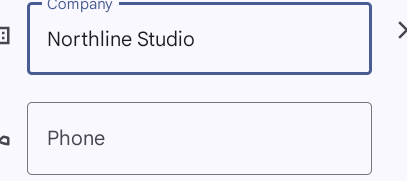
\includegraphics[width=.435\linewidth]{../docs/company-detail.png}\hspace{.04\linewidth}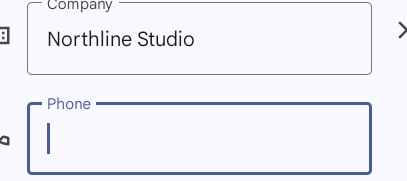
\includegraphics[width=.435\linewidth]{../docs/phone-detail.png}\\[-1pt]
\small (a) Before the tap \hspace{.20\linewidth} (b) After the tap
\end{center}
{\small\textbf{Figure 1.} Matching crops from the fastest child's recorded frames. The verifier decodes the full 480$\times$854 PNG, samples the actual field bounds from the live hierarchy, and checks for blue under Phone and its absence under Company.}
\hd{4\quad Results}
The six native-touchscreen requests on the same four-vCPU checkpoint took 1.328, 1.252, 1.154, 1.271, 1.215 and 1.145\,s in execution order. All passed. Their median was 1.233\,s, computed before rounding. In the same alternating series the first Android-dispatched gesture launch of a newly staged executable took 14.511\,s. First-launch effects matter when interpreting repeat-launch results. Ordinary OS caches were left enabled.
\begin{center}\begin{tabular}{@{}lrrr@{}}\toprule
Individual request & Guest connected & Remaining & Total \\ \midrule
Earlier two-vCPU software-rendered request & 1.083 & 2.407 & 3.490\\
Optimized two-vCPU software-rendered request & 0.505 & 1.065 & 1.570\\
Four-vCPU hardware-rendered minimum & 0.468 & 0.677 & 1.145\\ \bottomrule
\end{tabular}\end{center}
{\small\textbf{Table 1.} Times in seconds. Rows are individual observations. The four-vCPU fixture was saved separately with hardware rendering. Differences across rows include configuration and run-to-run effects.}
\par In a separate comparison, five alternating pairs used the same two-vCPU checkpoint. The original path passed 5/5 with a 3.271\,s median. A native-input variant polling the host renderer concurrently passed 4/5, with a 2.544\,s median among passes. One optimized attempt closed its observation stream without establishing the focus change. This matched comparison used a different capture schedule from the fastest touchscreen trial.
\newpage
\hd{5\quad Where the time went}
On the original 3.490\,s request, about 242\,ms elapsed from starting to load gfxstream to entering the renderer. A native stack sample traced work to dyld symbol resolution. Keeping dynamic lookup for unresolved host symbols and using two-level lookup for the renderer's other references reduced the observed repeat library load to about 5\,ms. Supplying the identical SDK kernel already decompressed reduced early setup work. An optional explicit SDK ADB path probes one executable and falls back to ordinary discovery on failure.
\par On an instrumented replay using the original observation path, Android reported gesture completion 0.302\,s after the guest observer began handling the request. It found Phone focused at 0.874\,s. The screenshot callback arrived at 1.249\,s and PNG encoding finished at 2.090\,s. Tree serialization overlapped capture. Guest stages use a separate monotonic clock. Reading the full emulator framebuffer on the host removes the guest bitmap copy and encoding from the winning path.
\par On the fastest request, 392\,ms separated sending the tap from receiving the tree. Another 265\,ms elapsed through screenshot acquisition and host verification. A different child showed the correct pixels as early as 742\,ms but returned the tree at 1.526\,s. Combining milestones from different children would understate latency. No complete trial established a subsecond verified tap.
\hd{6\quad Interpretation and reproducibility}
The experiment measures one local child and one deterministic first action in Contacts. It does not estimate simultaneous fan-out, throughput, long-horizon policy performance, arbitrary app restore fidelity, or cost on another host. No commercial environment was benchmarked. The checkpoint includes an observer configured in advance. Isolation checks saved a contact in a child after timing and reopened the sealed checkpoint to check its original unsaved state and focus. These checks establish isolation for the exercised draft.
\par The repository includes the emulator patches, upstream revision manifest, instrumented observer, runner, per-request timings, original full-resolution frames and accessibility XML. The \href{https://github.com/nikitph/droidfork/tree/main/experiments/fresh-restore}{build and fixture recipe} describes creating the source checkpoint and performing the measurement. The \data{fresh-profile/host-fixed-adb.json}{four-vCPU run file} contains every request in the headline series. The \data{FRESH-PROFILE.md}{profiling report} links the paired controls, failures and alternative capture strategies.
\hd{References}
[1] Android Developers. \href{https://developer.android.com/studio/run/emulator-snapshots}{Snapshots in the Android Emulator}.\par
[2] Android Open Source Project. \href{https://android.googlesource.com/platform/external/qemu/+/bbaa8072362a251645b339b97a737a725c776126/}{Emulator QEMU source, revision \texttt{bbaa8072362a}}.\par
[3] Apple Developer Documentation. \href{https://developer.apple.com/documentation/hypervisor}{Hypervisor framework}.
\end{document}
